\documentclass[twocolumn]{article}
\usepackage{listings} %for listing code
\usepackage{multirow} %multirow cells in tables
\usepackage{geometry}	%
\usepackage{abstract} %to get email footnotes
\geometry{margin=2cm}	%more visible figures (more place) 
\usepackage[superscript,biblabel]{cite}%superscript citing
\usepackage[utf8]{inputenc}
\usepackage[english]{babel}
\usepackage{amsmath}	%booklet
\usepackage{hyperref}	%clickable citings, referencing URL via \url{}
\usepackage{siunitx}	%for SI units; see ftp://ftp.dante.de/tex-archive/macros/latex/exptl/siunitx/siunitx.pdf
\usepackage{graphicx} 	%includegraphics
\usepackage{mhchem}		%writing chemical elements with mass numbers
\usepackage[nottoc]{tocbibind}	%references
\usepackage{indentfirst}%indenting first paragraphs
\usepackage{slashed} % for slash ET

%set code style

\lstset{		language=C++,
				frame=tb,
                basicstyle=\footnotesize\ttfamily,
                keywordstyle=\color{blue}\ttfamily,
                stringstyle=\color{red}\ttfamily,
                commentstyle=\color{green}\ttfamily,
                morecomment=[l][\color{magenta}]{\#},
                numbers=left
}


%the command \insertFigure{file} inserts figure with width 0.9*(column width)
\newcommand{\insertFigure}[1]{%
   \includegraphics[width=0.95\linewidth]{#1}%
}

\title{\textbf{E214: ATLAS}}
\author{Bence Mitlasóczki\thanks{s6bemitl@uni-bonn.de} and Beno\^it Scholtes\thanks{s6bescho@uni-bonn.de} \\ \textit{Rheinische-Friedrich-Wilhelms Universit\"at Bonn}}
\begin{document}
\renewcommand{\abstractname}{\vspace{-\baselineskip}} %supresses abstract title
\twocolumn[ %makes a one column abstract
\begin{@twocolumnfalse}
\maketitle
\begin{abstract} \vspace{-8mm}
Abstract goes here
\end{abstract}
\end{@twocolumnfalse}
\hspace{5mm} ]
\maketitle
\saythanks %from abstract package to ensure email footnotes from \thanks command in a two-collumn article
\section{Introduction}
Introduction text

The ATLAS detector is one of the several detectors in the LHC, a circular accelerator in Geneva, Switzerland. In it, two proton beams with the energy of 6.5~TeV each are collided with each other. The resulting legion %horde? multitude?
of particles are detected by the detectors. Out of these, the ATLAS (\textbf{A} \textbf{T}oroidal \textbf{L}HC \textbf{A}pparatu\textbf{S}) is the largest, general-purpose apparatus, able to detect the various particles created by the collisions. 

%TODO introduce acronyms: LHC
\section{Theory}
Our current best understanding of particle physics is the Standard Model of particle physics (SM). This model describes our discoveries of fundamental particles and their interactions with each other, mediated by fundamental forces. It furthermore describes the way these particles and forces combine to form atoms, from which many of the physical phenomena we encounter in everyday life can be explained. The main shortcoming of the SM however, is its inability to be united with gravity. That said, due to the relative weakness of gravity in comparison to the other fundamental forces, it rarely has an effect in particle physics and thus is mainly ignored (also in this experiment).

\subsection{The Standard Model}
Figure~\ref{fig:part} give a summary of the particles in the SM with their most basic properties. Furthermore, there also exists anti-particles of many of these particles. An anti-particle, such as a positron, is identical to its particle (electron) apart from having the opposite electric charge. A neutral particle is often its own anti-particle such as the $Z^0$~boson, though neutrinos have anti-particles which are merely distinct by having opposing spin projections. All matter particles and the W~bosons have anti-particles while the rest are their own anti-particles.
\begin{figure}[!h]
	\centering
	\insertFigure{Images/SM.png}
	\caption{Illustration of the elementary particles in the SM. Quarks are in purple and Leptons in green, arranged into generation columns from left to right. The gauge bosons are in red, with the scalar Higgs boson in yellow.~\cite{part}}
	\label{fig:part}
\end{figure}
Quarks and leptons make up all the matter particles that have been discovered. These are given in three generations of particles, shown with the columns from left to right in the figure. Matter that is encountered everyday is largely structured from the first generation, namely the electron, electron neutrino, up quark, and down quark. For example, atoms are made up of electrons, protons, and neutrons, the latter two being composed of up and down quarks. The second and third generations are composed of particles which are otherwise exactly identical to their first generation counterpart apart from being heavier, the third generation being the heaviest of them all. This is only known to be true for the charged leptons (electron, muon, and tau) and quarks however. Though the neutrinos are known not to be massless, they have very small masses which have not been accurately measured. It is unknown which is the most massive and which the least.~\cite{Thompson} Figure~\ref{fig:mass} illustrates the relative masses of the matter particles.
\begin{figure}[!h]
	\centering
	\insertFigure{Images/mass.png}
	\caption{Illustration of the relative masses of the matter particles in their respective generations. The neutrinos are left blank to show that their masses are extremely small in comparison the other particles.~\cite{Thompson}}
	\label{fig:mass}
\end{figure}
The main reason why the second and third generation of particles are largely not existent in everyday phenomena is due to the requirement that higher energies are needed to produce these heavier particles. Furthermore, these heavier particles have shorter lifetimes due to their favourable decay into lighter particles, such as those in the first generation, due to the fundamental tendency of physical systems to higher kinetic energy states. Particle physics experiments need to be performed at increasingly higher energies in order to produce more massive particles that we do not readily observe. This is illustrated in Figure~\ref{fig:energy}. It should be noted that though neutrinos are not seen, trillions of solar neutrinos pass through your body each second, oscillating between their three different flavours.~\cite{Thompson} They are extremely difficult to detect due to the fact that they have a small mass and no electric charge. \\
\begin{figure}[!h]
	\centering
	\insertFigure{Images/energy.png}
	\caption{Illustration of the energies required to probe different structures and particles.~\cite{Thompson}}
	\label{fig:energy}
\end{figure}
\par Figure~\ref{fig:part} also shows the fundamental forces in the SM which are all mediated via the exchange of a gauge boson. The most familiar of these is the photon $\gamma$ which mediates the electromagnetic force. The photon interacts with all particles that have an electric charge and thus with all fundamental matter particles in the SM apart from the neutrinos. It also interacts with the W~bosons as they are electrically charged. The gluon gauge bosons mediate the strong force, thus called as it is the strongest force and binds nuclei and hadrons together, explained in Section~\ref{sec:hadrons}. The gluons interacts only with particles which have a so-called ``colour" charge, another property of particles similar to electric charge. Only quarks have a colour charge and the eight differently coloured gluons. Next, the oppositely charged W$^{\pm}$ and Z$^0$~bosons mediate the weak interaction, the weakest force apart from gravity. This force is responsible for radioactive decay and interacts with all matter particles in the SM. Finally, the Higgs boson is the most recently discovered particle which gives mass to all the matter particles in the SM by interacting with them.

\subsection{Hadrons and the Strong Force}\label{sec:hadrons}
Though quarks are elementary in the SM, they cannot be observed as free particles. This is because quantum chromodynamics (QCD) of the SM, the theory of the strong force, states that colour is confined such that systems with a colour charge cannot propagate freely, termed \textit{colour confinement}. Instead, only colourless composite particles can be observed. As a result, quarks form composite particles called hadrons which are bound by gluons. Hadrons generally form baryons, composed of three quarks, and mesons, composed of one quark and one anti-quark. The reason for the these two types is a result of there being three colours, red, blue, and green, for the quarks, and three anti-colours, anti-red, anti-blue, and anti-green, for the anti-quarks. Colourlessness is achieved by combining all three colours (or anti-colours) in a baryon, or a colour and its anti-colour in a meson, as shown in Figure~\ref{fig:colour}. Protons and neutrons are examples of baryons, composed of two up quarks and one down quark (written as uud), and two down quarks and one up quark (udd), respectively.
\begin{figure}[!h]
	\centering
	\insertFigure{Images/colour.png}
	\caption{Colour confinement resulting in baryons and mesons, given with some examples.~\cite{colour}}
	\label{fig:colour}
\end{figure}
Furthermore, exotic hadrons, which achieve colour confinement with more quarks, have been hypothesised and observed, though without explicit confirmation that the observations were indeed bound exotic hadrons~\cite{Thompson}. Examples include the tetraquark with two quarks and two respective anti-quarks, and the pentaquark with four quarks and an anti-quark. Exotic hadrons are rare however, due to the tendency of quarks to form and decay quickly into mesons and baryons.

\subsection{The Structure of Protons} 
The inner workings of hadrons need to be properly considered to accurately model hadronic interactions, expanding on the simplifications of the previous section. Importantly, there does not merely exist three \textsl{valence quarks} in baryons, those required to achieve colourlessness. Rather, the binding gluons also split into $q\overline{q}$ pairs, producing extra quarks called \textsl{sea quarks}~\cite{manual}. These gluons and sea quarks then carry part of the baryons momentum and it is these \textsl{partons} that interact with other particles. Figure~\ref{fig:parton} shows this phenomena in a proton-proton interaction.
\begin{figure}[!h]
	\centering
	\insertFigure{Images/parton.png}
	\caption{Feynman diagram of proton-proton collision, namely between a valence quark (top) and a sea quark. The two produced gluons here will immediately \textsl{hardonise}, form into hadrons, as a result of colour confinement. Thus, this interaction produces two protons and two hadron jets.~\cite{manual}}
	\label{fig:parton}
\end{figure}
In order to model collisions accurately, such as the proton-proton collisions at the LHC, the kinematics of the partons need to be used, derived from parton distribution functions (PDF). These functions describe relative momentum of the different partons as a fraction of the baryon's momentum. They are determined from experiments and depend on the energy scale of the interactions. At the energy scale of the LHC, most proton-proton interactions are of their sea quarks and not valence quarks~\cite{manual}. One needs to consider all possible reactions however and observe the products of the interaction, such as the number of jets and their momenta, to identify an interaction in a collider experiment.

\subsection{The Heavy Gauge Bosons}%Citation is for the numerical data
\subsubsection{Production, Detection}
The three massive gauge bosons in the Standard Model are the neutral Z$^0$ and the charged W$^\pm$ bosons. The Z$^0$ boson has a mass of $91.1876 \pm 0.0021$~GeV~\cite{manual}. Its main decay mode is through jets ($\approx 70\%$). For our purposes, the decay to a lepton-antilepton pair (each lepton flavour having a branching ratio of $\approx 3.6-3.7 \%$) is the important mode, as it is easier to work with lepton tracks than jets. This is due to the large number of background QCD jets which are hard to distinguish from the Z$^0$ decay jets. The W$^\pm$ bosons have a slightly smaller mass of $80.403 \pm 0.029$~GeV, and they also decay to jets with the highest probability ($\approx 68 \%$), though the lepton-lepton ($e$, $\mu$) antineutrino decay modes are looked for in the experiment (the branching ratios are $\approx 10.6-11.3\%$ for each flavour) again due to their easy identification in the data. Both the W and Z bosons are produced in the weak Drell-Yan process, shown in Figure \ref{fig:WDiagram}.
\begin{figure} [!h]
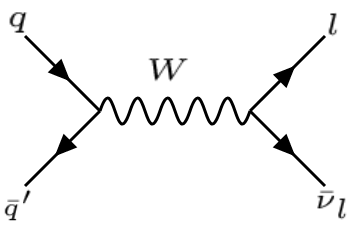
\includegraphics[scale=0.33]{Images/WDiagram.png}
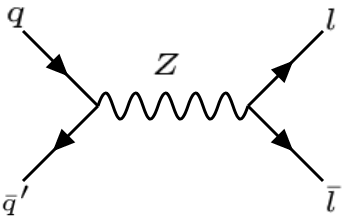
\includegraphics[scale=0.33]{Images/ZDiagram_differentflavour.png}
\caption{W and Z boson production and decay via the Drell-Yan process, from the interaction of a quark and anti-quark (not necessarily of the same flavour).}
\label{fig:WDiagram}
%Made with https://feynman.aivazis.com/
\end{figure}
The $Z^0 \rightarrow ee/\mu\mu$ processes can be precisely reconstructed from the ATLAS data, although there is a (suppressed) background from QED Drell-Yan pairs. In the case of $W \rightarrow e \bar{\nu}_e/\mu \bar{\nu}_\mu$ decays, the neutrino is not detected and its momentum needs to be reconstructed from the missing transverse momentum, as neutrinos are the mainly the only particle undetectable by the ATLAS detector. Both the W and Z boson decays are two-body decays, thus in the rest frame of the boson, the daughter particles have opposite three-momenta. It is easy to derive the $p_T$ (transverse momentum) spectrum in this reference frame, and use the fact that it does not change under Lorentz boosts in the beam direction to get an approximate distribution. For the Z boson, its mass is well-known and can be used to calibrate the ATLAS calorimeter. Examining the $Z^0 \, \rightarrow \, ee$ events, the observed invariant electron-positron mass distribution can be fitted with an approximate Breit-Wigner function. The W-boson mass will be sought as explained below. %We will utilize the precisely known $Z^0$ mass for the verification of our method in Section~\ref{sec:Proc}, and consider the case of the W-boson mass below. 

\subsubsection{The Jacobi Peak} \label{sec:yo}
%TODO not entirely clear why are we looking at d(sigma)/d(pT) and not sigma(pT), maybe because we are looking at bins, thus dsigma  ~ d(sigma)/d(pT)*d(pT)?
%TODO Check bibliography item WMassExperiment (correct form?)
In the process $W \, \rightarrow \, l \bar{\nu}_l$, the final state leptons have an approximate angular distribution~\cite{manual}
\begin{equation}
\frac{d\sigma}{d\cos \theta^*} = 1 + \cos^2 \theta^*, \nonumber
\end{equation}
where $\theta^*$ denotes the angle between the lepton track and the beam axis.
With this knowledge, we can calculate the differential cross-section
\begin{equation}
\frac{d \sigma}{d p_T} = \frac{d \sigma}{d \cos \theta^*} \left\vert \frac{d p_T}{d \cos \theta^*} \right\vert^{-1} = \frac{d \sigma}{d \cos \theta^*} \cdot  \frac{\frac{2p_T}{M_W}}{\sqrt{\left( \frac{M_W}{2}\right)^2 - p_T^2}}. \nonumber
\end{equation}
This curve clearly has a pole at $p_T = \frac{M_W}{2}$, called the Jacobi peak, and there should be no events with $p_T > \frac{M_W}{2}$ in a decay of the W-boson at rest. In reality, there are three distorting effects. Firstly, the detector is made of multiple parts each having a different sensitivity, or even not working, contributing to somewhat imprecise measured (and missing) momenta. Secondly, the W-boson mass has a Breit-Wigner type distribution centred at $M_W$ as it is not stable. The $p_T$ distribution should reflect this as well. Thirdly, the W-boson at the tree level has no transverse momentum (this assumption is made to derive the formula above), but the radiative corrections allow for some initial $p_T$. An example process is shown in Figure \ref{fig:WRadiation}. 
\begin{figure} [!h]
\centering
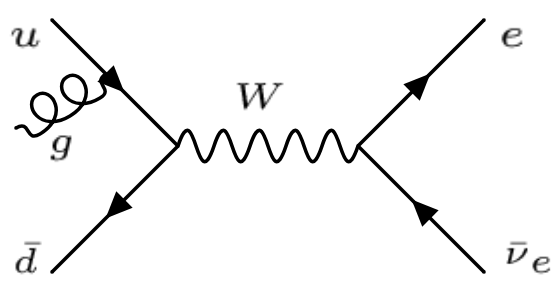
\includegraphics[scale=0.25]{Images/WRadiation.png}
\caption{Feynman diagram of a W-boson production with initial state radiation, giving the W-boson non-zero transverse momentum.}
\label{fig:WRadiation}
\end{figure}
\begin{figure} [!h]
\centering
\insertFigure{Images/WmassExample.eps}
\caption{An example of the expected electron transverse momentum histogram.\cite{WMassExperiment}}
\label{fig:WmassExample}
\end{figure}
In the ideal case, one can easily declare the measured mass as the peak in the histogram. The distorting effects however smoothen out the curve complicating things, as seen in Figure \ref{fig:WmassExample}. The alternate method used to calculate the W~boson mass will be explain in Section~\ref{sec:Wmass} alongside the results obtain from this method.

\iffalse
\subsection{$Z^0$-Pair Production} %TODO I'm not sure about this section, it doesn't read well and doesn't really fit in to the report. Maybe put it after the next section or get rid of it. It doesn't go into enough detail to make it understandable.
Although we chose to determine the mass of the W-boson, here follows a short description of the other main task, searching for new physics phenomena in simulated data. The place to look in this case is the set of events where a $Z^0$ pair decays into four leptons, as this gives a clear signal of a ZZ event. The task here is to get rid of background events; these are a $t \bar{t}$ pair decaying via $t \rightarrow b W^+ \rightarrow b \, l^+ \nu_l$, or a Z boson with two additional b quarks (in both cases, B-hadrons that contain the b quarks might decay semi-leptonically, producing one more lepton each) with the help of data sets containing such events. After getting satisfactory filtering, a data set with SM and simulated Higgs or other "new physics" events; by looking at the characteristics of each hypothetical scenario (SUSY in the form of $Z Z^{(*)}$ events, new generation quarks, or additional gauge bosons ($Z^\prime$)), we need to decide which one might have appeared in the experiment.
\fi
\subsection{Extensions to the SM}
Though the SM has been extremely successful at describing fundamental physics, it has several shortcomings which necessitate explanations from new physics. Of these, some of the most significant are the inability of the SM to explain neutrino oscillations, gravity, dark matter, and the hierarchy problem. The latter is the observed discrepancy between the strengths of the fundamental forces. The strengths are quantified by coupling constants of the relevant gauge bosons with the relevant charge (gluons with colour charge) and these ``constants" actively depend on the energy scale of the interactions. That said, if a grand unified theory (GUT) of the three fundamental forces is to be established, whereby the forces are unified at some higher energy scale, it is expected that the strengths of the different coupling constants converge at this scale, a phenomena which is seemingly not achieved within the SM. \\
\par There are numerous theories which attempt to solve the different problems of the SM. One more promising theory is supersymmetry (SuSy) which proposes solutions to the hierarchy problem and provides a candidate dark matter particle. The minimal supersymmetric extension to the SM (MSSM) states that each lepton in the SM has a bosonic superpartner of spin 0, while every boson has a fermionic superpartner of spin 1/2. Figure~\ref{fig:susy} shows the MSSM particle spectrum.
\begin{figure}[!h]
	\centering
	\insertFigure{Images/susy.png}
	\caption{Particles in the MSSM.~\cite{susy}}
	\label{fig:susy}
\end{figure}
The superparticles have undefined mass, as MSSM particles of mass equal to their superpartners have not been found. As particle physics experiments such as the LHC have not found any MSSM particles yet, it is likely that they have much larger masses not probed yet by the LHC, if MSSM is indeed accurate. MSSM introduces a conserved and multiplicative quantum number called R-parity, defined as $R = (-1)^{3B+L+2S}$, where $B$ is baryon number, $L$ is lepton number, and $S$ is spin. SM particles have +1 R-parity while superparticles have -1 R-parity. As a result, a superparticle cannot decay into SM particles without violating R-parity. Thus, the lightest supersymmetric particle (LSP) must be stable. This is the natural dark matter particle candidate introduced by SuSy. Furthermore, with SuSy the three fundamental force coupling constants do indeed approximately unite at a scale of $10^{16}$~GeV, solving the hierarchy problem. Searching for evidence of SuSy is currently one of the main goals of the LHC as this would be a major leap in our understanding of physics. As of yet, no such signature have been observed. Other searches of new physics include additional heavy bosons proposed by other SM extension theories, such as bosons similar to the Z boson yet heavier. Furthermore, searches of higher generations of quarks and leptons in the SM are also conducted since they could very well exist yet are so massive that they have not been able to be produced in particle collisions. The LHC can easily investigate such proposals yet is limited in the energy of collisions and thus the masses of the produced particles.

\section{The ATLAS Detector}\label{sec:Exp}
This experiment analyses data from the ATLAS detector at the LHC. The ATLAS detector is cylindrical in shape, where the proton beams enter through each end of the cylindrical detector and collide in its centre. It makes use of numerous layers in order to detect particles produced in the collisions. Figure~\ref{fig:ATLAS} is a cross-sectional perspective of the detector showing the different layers. Circular detector disks are also added to the two ends of the cylindrical detector to further detect and measure particles at small angles to the beam axis.
\begin{figure}[!h]
	\centering
	\insertFigure{Images/ATLAS.png}
	\caption{Cross-sectional view of the ATLAS detector showing the different detectors at different layers and how different particles interact with the detectors. Most of the muon spectrometer is not included in this image.~\cite{manual}}
	\label{fig:ATLAS}
\end{figure}

\subsection{Inner Detector}
The inner detector helps determining the particle paths as precisely as possible. A solenoid magnet surrounds this system, creating a $\vec{B} = 2$~T magnetic field parallel to the colliding protons so as not to deflect them before collision. A particle with charge $q$ and velocity $\vec{v}$ in this magnetic field experiences a Lorentz force of 
\begin{equation}
\vec{F} = \frac{d}{dt} \vec{p} = q \vec{v} \times \vec{B}.\nonumber
\end{equation}
From the observed radius of the track of the particle, its momentum and charge sign can be determined allowing for a kinematic analysis of the collision. One can see in Figure~\ref{fig:ATLAS} how the charged particles are bent by the magnetic field in the inner detector. The inner detector is composed of different layers of detectors, hereby summarised:
\begin{itemize}
\item The innermost layer consists of over 80 million silicon semiconductor pixels (pixel detector, PD) which each have their own electronic circuit.~\cite{manual} This allows for precise spatial reconstruction of vertices, importantly being able to distinguish between closely separated primary and secondary vertices.
\item The semi-conductor tracker layer (SCT) serves the same purpose, but with long strips that make covering a larger surface area more practical.
\item The transition radiation tracker (TRT) consists of thin, long tubes (drift chambers) with inhomogeneous medium filling in the space between them. A particle passing through this medium emits transition radiation. The photons created this way, along with the particle itself, interact with the gas inside the tubes, causing ionizing. As there is a voltage applied to an electrode in the middle and the tube, the electrons are drawn to the electrode, contributing to an electric pulse. As the transition radiation is strongest for particles with high velocity, the strength of the signal can be used to identify the lightest particles, electrons and positrons.
\end{itemize}

\subsection{Outer Layers}
The layers surrounding the inner detector are largely used to determine the energies of the particles. It is composed of three sections.
\subsubsection{Electromagnetic Calorimeter}
The electromagnetic calorimeter (ECAL) is made of accordion-shaped lead and stainless steel sheets responsible for interacting electromagnetically with the particles passing through, creating an electromagnetic shower, seen in Figure~\ref{fig:ATLAS}. The liquid argon between the lead and steel sheets is ionized by the particles passing through, and the created free electrons are drawn to a copper electrode. An electromagnetic shower is caused by the radiation emitted from bremsstrahlung and compton scattering of the charged particle, whereby the emitted photons then pair-produce, which themselves emit radiation. This cycle continues until photons are emitted which aren't energetic enough to pair-produce. The shower of electron, positron, and photons produced are the electromagnetic shower, which deposits its energy in the detector allowing for a determination of the original particles energy. This calorimeter stops photons, electrons and positrons entirely and single handedly allows for a calculation of their energies. Hadrons and muons also deposit some energy here, but they pass through to reach the outer layers. The cooling system is a cryostat.

\subsubsection{Hadron Calorimeter}
The hadron calorimeter (HCAL) interacts strongly with the entering particles. The iron tiles induce hadronic showers, identical to the electromagnetic showers but caused hadrons colliding inelastically with the nuclei of the calorimeter material. The particles thus created enter the scintillation tiles producing light, and these photons are carried away in an optical fibre to a unit which measures light intensity, from which the deposited energy can be calculated. The scintillation material is liquid argon, so a cooling system is used in this layer as well. This calorimeter stops all hardons, leaving only muons and neutrinos to escape this layer of the detector.

\subsubsection{Muon Spectrometer}
The muon spectrometer is needed to measure the energy of the muons. The muons are so massive that they don't emit bremsstrahlung and don't interact strongly meaning that they only deposit a small amount of their energy in the previous layers of the detector. This unit is supplemented by a larger magnetic system consisting of toroidal magnets such that the detector is capable of determining the momentum of the muons independently of the inner layers. The tiles making up this layer consist of thin tubes filled with gas, and work on the principle of ionization, similarly to the TRT tubes. 

\section{Procedure and Results} \label{sec:Proc}
\subsection{ATLANTIS}
As our first task, we looked at examples of events in the ATLAS detector in the event display software ATLANTIS. This way we got familiar with the working of the ATLAS detector and the signatures of different particles in the detector.
\begin{figure} [!h]
	\centering
	\insertFigure{Images/Atlantis_Electron_cropped.png}
	\caption{An (artificial) electron track as viewed in ATLANTIS, showing the electromagnetic shower (yellow) in the ECAL (green). The panel with quantitative information and control functions has been cropped for better visibility.}
	\label{fig:elec}
\end{figure}

\subsubsection{Electron Energy}
We looked at the first 24 electron events in the learning data-set, determining the momentum by the track radius and the energy of the ECAL clusters by manually selecting the region. Figure~\ref{fig:elec} shows an example of an electron signature in ATLANTIS. The results are summed up in Table~\ref{tab:electron}. The histogram made of the energy/momentum ($E/p$) ratios is shown in Figure~\ref{fig:electron_histogram}. 24 events were chosen as four events were inconclusive as energy was not deposited, leaving 20 meaningful events.
\begin{figure} [!h]
\centering
\insertFigure{Images/electron_histogram.png}
\caption{Electron E/p histogram.}
\label{fig:electron_histogram}
\end{figure}

\begin{table} [!h]
\centering
\begin{tabular}{|c|c|c|c|}
\hline
\# & Momentum (GeV) & Energy (GeV) & E/p\\
\hline
1&	26.2&		54.7&	2.09\\\hline
2&	22.78&		35.2&	1.55\\\hline
3&	244.35&		223.2&	0.91\\\hline
4&	N/A &		N/A&	N/A\\\hline
5&	N/A	&		N/A&	N/A\\\hline
6&	66.67&		78.3&	1.17\\\hline
7&	7.55&		56.6&	7.50\\\hline
8&	129.82&		162.9&	1.25\\\hline
9&	3.27&		47.7&	14.59\\\hline
10&	79.01&		66.2&	0.84\\\hline
11&	95.93&		78.7&	0.82\\\hline
12&	37.4&		30.6&	0.82\\\hline
13&	89.35&		86.5&	0.97\\\hline
14&	235.24&		242.3&	1.03\\\hline
15&	105.14&		105.3&	1.00\\\hline
16&	N/A	  &		N/A&	N/A\\\hline
17&	28.62&		28.1&	0.982\\\hline
18&	53.41&		46.4&	0.869\\\hline
19&	32.92&		64.3&	1.95\\\hline
20&	105.64&		80.8&	0.765\\\hline
21&	N/A	  &		N/A&	N/A\\\hline
22&	93.52&		82.1&	0.878\\\hline
23&	113.98&		92.7&	0.813\\\hline
24&	155.35&		283&	1.82\\\hline
\end{tabular}
\caption{The momenta and energies of electrons, determined by the inner detector and ECAL, respectively. The E/p values are subsequently calculated.}
\label{tab:electron}
\end{table}
From the data, it can be seen that quite a few electrons were measured to have slightly higher momentum than energy, indicating the inaccuracy of the detector. The histogram shows that most electrons were measured with similar energy and momentum, as expected, though two relativistic electrons are found with E/p=7.50 and 14.59, identified due to their much larger energy than momentum detected. Their momentum is much smaller due to their inaccurate calculation from their rest mass, as opposed to relativistic mass, with their radius in the inner detector. A larger sample is required to determine the proper E/p distribution of electrons and whether a higher ratio of relativistic electrons are produced.

\subsubsection{Muon Momentum Comparison}
As our second task, we compared the measured muon momentum in the muon spectrometer and the inner detector. Calculating the differences between the two methods allowed us to determine the energy loss of the muons in the calorimeter and whether this depended on any quantity of the muons, such as their direction of flight. Table~\ref{tab:muon} provides the results. Figure~\ref{fig:muonat} shows a muon event in ATLANTIS.
\begin{table} [!h]
\centering
\begin{tabular}{|c|c|c|c|c|c|}
\hline
\multirow{2}{*}{\#} 	& I.D.		& M.C. 		& Diff. 	& \multirow{2}{*}{$\eta$} & \multirow{2}{*}{$\phi^{\circ}$}\\
					& (GeV)	& (GeV)	& (GeV)	&	&\\
\hline
1&	85.28&		53.92&		31.36&		1.437&	21\\\hline
2&	43.4&		43.83&		-0.43&		-0.767&	25\\\hline
3&	241.37&		237.02&		4.350&		-2.438&	230\\\hline
4&	48.89&		44.77&		4.12&		0.567&	311\\\hline
5&	168.16&		177.62&		-9.46&		-1.809&	244\\\hline
6&	117.32&		96.56&		20.76&		1.621&	152\\\hline
7&	71.94&		64.96&		6.98&		0.699&	3.8\\\hline
8&	199.91&		199.44&		0.470&		1.797&	67\\\hline
9&	57.84&		50.01&		7.830&		-0.287&	241\\\hline
10&	71.1&		0&			71.1&		1.181&	312\\\hline
11&	100.75&		94.11&		6.64&		-1.636&	48\\\hline
12&	38.26&		34.48&		3.78&		0.189&	326\\\hline
13&	105.19&		108.68&		-3.490&		1.163&	224\\\hline
14&	236.12&		263.61&		-27.49&		2.286&	103\\\hline
15&	131.69&		125.51&		6.180&		-1.763&	255\\\hline
16&	152.24&		157.69&		-5.450&		-1.874&	27\\\hline
17&	35.23&		32.18&		3.05&		0.395&	326\\\hline
18&	54.19&		50&			4.19&		0.229&	336\\\hline
19&	84.75&		68.09&		16.66&		0.773&	260\\\hline
20&	104.26&		107.98&		-3.72&		1.421&	78\\
\hline
\end{tabular}
\caption{The first column shows the Inner Detector measured momentum values, the second column the muon calorimeter momenta, the third column the loss of momentum (negative values show an increase in momentum), the fourth column $\eta$, the pseudorapidity, and the last column the azimuthal angle with respect to the proton beam axis. Uncertainty is not herein included as it was not insightful to the investigation of quantity dependence on energy difference.}
\label{tab:muon}
\end{table}
Here, we found that there are some cases where the muons seem to have gained momentum. This is indicative of the fact that the momenta of the muons are not accurately calculated in the inner detector due to the short pathlength of the muon in the detector and the insignificant deflection of the muon due to its large mass. As a result, the radius of the muon's arc cannot be precisely measured, thus resulting in an inaccurate measurement of the muons momentum. The muon system is much larger, on the other hand, allowing for a much more precise calculation of the muon momenta. Ultimately, the average energy loss of the muons in the calorimeter is 6.87~GeV. The possible dependence of the energy loss of the muons on their pseudorapidity $\eta = -\ln(\tan(\theta/2))$ ($\theta$ being the polar angle) and their azimuthal angles $\phi$ was analysed. These quantities were chosen as they were determined to be the only reasonable quantities that the measured energy loss could depend on. It was reasoned that the ends of the ATLAS detector, which are fitted with detector plates in which the calorimeters and muon system don't extend as far as in the middle cylindrical section, won't be able to measure the muon momenta as accurately, or that the muons won't dispose as much energy in the shortened calorimeter. That said, no dependence on these quantities was found in the energy loss of the muons. This could either be because there is no such correlation to be found or that a large sample size is required. A larger sample size could be needed as the accuracy of the measured muon momenta is not very high, resulting in fluctuations in the energy differences calculated which obscure any $\eta$ or $\phi$ dependence. A large sample size could counteract this obscurity.
\begin{figure} [!h]]
\centering
\insertFigure{Images/Atlantis_Muon_cropped.png}
\caption{Artificial muon event as seen in ATLANTIS. Slight energy deposition in the HCAL can be observed. The detector view is in fisheye mode so that the size of the muon system is reduced to allow for better visibility of the more central detectors.}
\label{fig:muonat}
\end{figure}

\subsection{ECAL Calibration}
The energy data obtained from the ECAL detector needs to be properly calibrated to give the correct energies of particles. This will allow for a more accurate measurement of the energies of the detected leptons used to measure the mass of the W-boson in the next section. The raw output energies are not accurate as the ECAL is composed of many modules which all have slightly different sensitivities, or may even be inactive, resulting in varying energy outputs. Furthermore, the particles can lose energy before reaching the ECAL and calibration can counteract any such systematic offset. Ultimately, different regions of the ECAL need to be calibrated differently, corresponding to the different raw sensitivities and inactivities of those regions. We made cuts of the pseudorapidity and azimuthal angle to probe different regions and calibrated their energies individually. We chose sections with widths of $\Delta \eta = 1.25$ and $\Delta \varphi = \pi/2$, over the full range of the detector: $-2.5 \leq \eta \leq 2.5$ and $-\pi < \varphi < \pi$. The $\eta$ and $\phi$ cuts were made simultaneously, so as to probe more localised regions of the detector, as opposed to slices in $\phi$ and $\eta$. This was deemed to be a more sensible approach as we reasoned that discrepancies in the detector are more likely to be localise to smaller areas as opposed to be dependent individually on $\eta$ or $\phi$. If this was not the case however, our simultaneous cuts of $\phi$ and $\eta$ would still be able to detect individual dependence on these angles. To reduce computational time, however, the number of cuts made in $\phi$ and $\eta$ individually could not be as many as if we had made the cuts separately, thus not probing the individual dependence finely. Further experimentation should determine whether making cuts in $\phi$ and $\eta$ individually more effectively calibrates the detector than simultaneous. \\
\begin{figure} [!h]
	\centering
	\insertFigure{Images/ElectronEnergyLabeled.png}
	\caption{Histogram of energy of electrons from Z$^0$ decays, with the peak at $\sim$ $m_{Z^0}/2$.}
	\label{fig:Elec}
\end{figure}
\begin{figure} [!h]
	\centering
	\insertFigure{Images/PositronEnergyLabeled.png}
	\caption{Histogram of energy of positrons from Z$^0$ decays, with the peak at $\sim$ $m_{Z^0}/2$.}
	\label{fig:Pos}
\end{figure}

\par In addition to probing different regions of the ECAL, separate cuts on the momenta of the particles were made. This was to determine whether there was any dependence of the inaccurately measured particle energies with their momenta calculated in the inner detector. This could be caused by the ECAL reacting non-linearly to different momenta of the particles, resulting in inaccurate energy measurements. To calibrate the detector, electron-positron pairs from Z$^0$~boson weak decays were used as the mass of the Z$^0$~boson is very precisely known. Furthermore, the Z$^0$~boson are produced with insignificant transverse momentum due to the collinearity of the protons and thus partons which create them. This means that the invariant mass of the produced electron-positron pair is equal to the Z$^0$~boson mass and thus is very finely set. To calibrate the detector, the invariant mass of the $e^-e^+$ pair was calculated for each cut to determine its discrepancy from the Z$^0$~boson. The energy yield of that cut was then multiplied by $m_{Z^0}/m_{\text{calc}}$ such that region of the ECAL should be calibrated to measure the correct mass for the Z$^0$~boson. Figures~\ref{fig:Elec},~\ref{fig:Pos}, and~\ref{fig:Inv} depict the electron energy, positron energy, and electron-positron invariant mass histograms, respectively, before a calibration was performed. It can be seen that the peaks of the histograms line up approximately with the ideal values of $m_{Z^0}/2$ for the first two, and $m_{Z^0}$ for the last one. This suggests that the ECAL is already quite well tuned to providing accurate energy yields, though not exactly, demonstrating the necessity for the calibration. The uncalibrated ECAL calculated a mass of the Z$^0$ of $89.87 
\pm 0.02$~GeV, demonstrating that, on average, the calibration needed to magnify the energy output of the ECAL detector.\\
\begin{figure} [!h]
	\centering
	\insertFigure{Images/InvMassLabeled.png}
	\caption{Histogram of invariant mass of the positron-electron pairs, with the peak at $\sim$ $m_{Z^0}$.}
	\label{fig:Inv}
\end{figure}
\par The Appendix, Section~\ref{sec:Code}, shows the code written for the calibration for use in the ROOT program of CERN. We attempted to iterate this process by again measuring the respective masses with the recently calibrated regions and then recalibrating the newly calculated mass discrepancies. This turned out to be counterproductive however, as the calculated Z$^0$~boson mass became less accurate. The reason for this is unknown but due to the fact that the originally calculated Z$^0$~boson mass was adequately accurate, the first calibration was merely taken for the rest of the experiment. Further experimentation can investigate different cuts, such as cutting the pseudorapidity and azimuthal angle separately to determine whether iterative calibrations work in that case, or if not, perhaps why they do not work. \\
\begin{figure} [!h]
	\centering
	\insertFigure{Images/FinalIterationLabeled.png}
	\caption{Histogram of electron-positron invariant mass with Voigt fit, giving the mass of the Z$^0$~boson at the position of the peak.}
	\label{fig:final_iteration}
\end{figure}
\par Ultimately, the mass for the Z$^0$~boson after our calibration was calculated by fitting a Voigt function to the electron-positron invariant mass $M_{ee}$ histogram, given in Figure~\ref{fig:final_iteration}. A Voigt function is a Breit-Wigner curve convoluted with a Gaussian. This is to be expected for the histogram as resonances (short-lived particles) have Breit-Wigner distributions, yet the inaccurate detector effects are Gaussian distributed. The optimally calculated Z$^0$~boson mass is $91.198 \pm 0.020$~GeV, in good agreement with the known value, giving confidence in our ECAL calibration.







\subsection{Measurement of the W-boson mass} 
\subsubsection{QCD Background Normalisation} \label{sec:QCD}
The main aim of this experiment is to use the previous calibration to measure the mass of the W~boson from real ATLAS data. The $W^- \to e^- + \nu_e$ and $W^+ \to e^+ + \overline{\nu_e}$ decays, shown in Figure~\ref{fig:WDiagram}, are herein analysed to determine the mass of the W~boson. Firstly, the ECAL calibration was tested on real ATLAS data of Z$^0 \to$ ee decays to determine whether the produced Z~boson mass agrees with world-averaged value. Different kinematic regions were tested to determine whether the calibration was consistent. Figure~\ref{fig:Z0ATLAS} gives the produced histogram when no cuts were made. The produced mass is $91.17 \pm 0.01$~GeV, in good agreement with the world average. All kinematic regions investigated were also in good agreement, suggesting that our ECAL calibration was functioning as desired.
\begin{figure}[!h]
\centering
\insertFigure{Images/FirstWFitLabeled.png}
\caption{Z$^0$ mass from ATLAS data}
\label{fig:Z0ATLAS}
\end{figure}
\par The next step was to normalise the QCD background to the size of our used ATLAS data for measuring the W~boson mass. The QCD background is all data that results from the colliding proton partons interacting strongly, in which the W~boson does not appear. As a result, this background complicates our analysis it dominates the data and yet cannot be used to measure the W~boson mass. In order to consider data which is more dominated by W~boson interactions, the QCD background needs to be approximated in the real ATLAS data used to measure the W~boson mass. This is achieved by extracting QCD background data from other ATLAS data to determine its shape and presence in different plots and kinematic regions. However, this applied QCD background firstly needs to be properly scaled to the size of the now used ATLAS data for the W~boson. This is achieved by looking at different plots of the ATLAS data, plotted with stack-plots of the simulated expected QCD background, non-QCD background, and $W \to e\nu$ (or $Z \to ee$) contributions. The plots investigated were the transverse momentum of detected electrons, the isolation energy of the electrons (summed energy in a cone around the electron), the missing transverse energy, the number of jets, and the estimated transverse momentum of the W~boson. Firstly, the scaling of the QCD background was altered such that the different simulated stack-plots agreed with the ATLAS data, observed by eye. Specifically, regions which had a QCD background contribution were dominant were focused on to try to scale the QCD background as accurately as possible. Figure~\ref{fig:QCDscalefactor} is one such plot of the estimated transverse momentum of the W~bosons, with the QCD scale factor changed such that the ATLAS data and stack-plot agree.
\begin{figure}[!h]
	\centering
	\insertFigure{Images/ptw_scaleLabeled.png}
	\caption{QCD scaled to 0.45 (initially 1.0) achieved a good match between the stack-plot and the data points, especially around the ${P_T}_W \approx 50$~GeV area where the QCD background is most dominant.}
	\label{fig:QCDscalefactor}
\end{figure}
Unfortunately, the scale factor obtain from this method for the different plots did not agree, where in Figure~\ref{fig:QCDscalefactor} it was 0.45, though for the missing transverse energy it was 0.40. \\

\par Ultimately, the W~boson mass will be measured using the transverse momentum of the electrons produced in the W~boson decays, explained later in this section. As a result, this plot was focused on and the scale factor was changed until stack-plot sections with high QCD background agreed with the ATLAS data. The scale factor hereby obtained was approximately 0.25-0.30. That said, this scale factor meant that the other stack-plots were not in good agreement with the ATLAS data, suggesting that it was not likely to be the correct scale factor for this ATLAS data and thus shouldn't be used. A compromise was chosen for the scale factor of $0.35 \pm 0.05$ such that all plots were in relatively good agreement with the data. It is unknown why there is a discrepancy between different plots for the optimal QCD scale factor, apart from the QCD background being merely a simulated, non-ideal estimation on the real QCD background in the data. The uncertainty in the scale factor was determined as the range of values which resulted in adequate agreement between the ATLAS data and the stack-plots in all the plots considered. \\

\par Next, cuts were made on the data to only include data which had low QCD and non-QCD background, in order to optimise the calculation of the W~boson mass. By looking at the different plots mentioned previously, the following cuts were made:
\begin{itemize}
\item transverse momentum of the W~boson $\textless$ 20~GeV,
\item isolation energy of the electron $\textless$ 4~GeV,
\item number of jets $\textless$ 2, and
\item 20 $\textless$ (missing transverse energy) $\textless$ 60.
\end{itemize}
The number of jets were taken to be at most one as the jets are caused from radiative corrections, shown in Figure~\ref{fig:WRadiation}, give transverse momenta to the W~boson thereby making the process of calculating its mass more complicated. One jet was allowed as only considering no jets reduced the data too much to obtain statistically significant results. The above cuts were those used for the following measurement of the W~boson mass.
	
\subsubsection{Gauge Curve Procedure} \label{sec:Wmass}
As mentioned in Section~\ref{sec:yo}, the W~boson mass cannot be calculated simply by locating the Jacobi peak, due to distorting effects. Instead, we take advantage of the seven available simulated data sets of $W to e\nu$ decays with different W~boson masses. For each, we can fit a polynomial function that takes into account the distorting effects of the Jacobi peak and find the half-maximum of the fit. This allows us to acquire a correlation between simulated W-boson mass and half-maximum values, to which a linear regression is applied. The resulting linear fit is called the gauge curve. Figure~\ref{fig:gaugecurve} shows the gauge curve we obtained, demonstrating a very linear relationship
\begin{figure}[!h]
	\centering
	\insertFigure{Images/Jacobihalfmax.png}
	\caption{The gauge curve data points with linear fitting, should very good agreement with the linear regression.}
	\label{fig:gaugecurve}
\end{figure}
\begin{equation}\nonumber
\text{HM}(m) = (0.5027 \pm 0.0087)\cdot m + (2.26 \pm 0.69)
\end{equation}
The fits of all seven simulated data sets are given in the Appendix, Section~\ref{sec:half}. Using the gauge curve and calculating the half-maximum corresponding to the real ATLAS W-boson data, we can obtain the real W-boson mass. We obtained a half-maximum for the real ATLAS data to be $43.04 \pm 0.09$~GeV, given in Figure~\ref{fig:halfW}, which gives a mass of W~boson of $m_\text{W} = 81.1 \pm 2.0$~GeV. 
\begin{figure}[!h]
	\centering
	\insertFigure{Images/WmassLabeled.png}
	\caption{Plot of the transverse momentum of electrons from real ATLAS W~boson decays with half-maximum fit overlayed. The previously mention cuts have been applied for this plot.}
	\label{fig:halfW}
\end{figure}
This value agrees well with the world-average value for the mass. That said, the uncertainty calculated in this value is quite large, largely derived from large relative uncertainty in the intercept value of the gauge curve. Further experiments should try to reduce this uncertainty, perhaps by using more simulated data sets, in order to obtain a more precise mass for the W~boson. Regardless, the calculated mass is in good agreement with the world-averaged value, giving confidence in our method.\\

\par As a further cross-check, we applied the half-maximum fit to electron transverse momenta from $Z^0$ decays to determine whether an adequate $Z^0$ mass was also obtained. Figure~\ref{fig:crosscheck} shows the corresponding plot. 
\begin{figure}[!h]
\centering
\insertFigure{Images/ZeeCheckLabeled.png}
\caption{Plot of the transverse momentum of electrons from Z~boson decays with half-maximum fit overlayed, used for the cross-check of our method.}
\label{fig:crosscheck}
\end{figure}
The resulting calculated mass using the gauge curve is $91.93 \pm 2.2$~GeV, again in good agreement with the world-averaged value. This gives further confidence that our method has accurately determined the mass of the W~boson from real ATLAS data. The large uncertainty here is again as a result of the uncertainty in the gauge curve.

\subsubsection{Sources of Systematic Uncertainty}
It is insightful to investigate any sources of (systematic) uncertainty in our methodology. The most obvious possible source of such uncertainty comes from the QCD background scaling. This is due to the large possible range of scale factors which agreed with different parts of the data, resulting in its large uncertainty. In Section~\ref{sec:QCD}, we obtained a scale factor of $0.35 \pm 0.05$. As a result, the method used in Section~\ref{sec:Wmass} was repeated for a QCD scale factor of 0.30 and 0.40, the edges of the uncertainty range. By calculating the resulting W~boson mass from these scale factors, we could quantify the systematic uncertainty introduced by the QCD background scaling method. Figures~\ref{fig:W1} and~\ref{fig:W2} give the half-maximum plots for the QCD scale factors of 0.30 and 0.40, respectively. 
\begin{figure}[!h]
	\centering
	\insertFigure{Images/Wmass_30Labeled.png}
	\caption{Plot of the transverse momentum of electrons from W~boson decays with half-maximum fit overlayed, for a scale factor of 0.30.}
	\label{fig:W1}
\end{figure}
\begin{figure}[!h]
	\centering
	\insertFigure{Images/Wmass_40Labeled.png}
	\caption{Plot of the transverse momentum of electrons from W~boson decays with half-maximum fit overlayed, for a scale factor of 0.40.}
	\label{fig:W2}
\end{figure}
It can be seen that the stack-plots in the two plots deviate slightly from the data, though not significantly enough to rule out the scale factor as inaccurate, demonstrating the source of the uncertainty. That said, the scale factor of 0.30 fits the data more accurately than that for 0.40, demonstrating the point made in Section~\ref{sec:QCD} about the scale factor approximated from the electron transverse momentum plot at 0.25-0.30 (though larger for other plots). Ultimately, however, the produced half-maximums from the fit are both exactly the same as that for the used scale factor in Section~\ref{sec:Wmass}. Thus, the QCD scaling has not introduced systematic uncertainty in the calculation of the W~boson mass. Given that the QCD background scaling was the most uncertain part of the method, in our opinion, this result has given us confidence that our calculation for the W~boson mass isn't very sensitive to the uncertain QCD scaling process. It furthermore demonstrates that our accurately measured mass isn't somewhat by chance, but that it is quite stable if the method is properly executed. Ultimately, it gives further confidence that our result for the W~boson mass is $81.1 \pm 2.0$~GeV.

\section{Conclusion}
The aim of this experiment was to familiarise ourselves with data analysis obtained at the ATLAS detector and ultimately, to calculate the mass of the W~boson from real ATLAS data. Initially, we investigated the signatures left by different particles in the detector with the ATLANTIS program. We determined from this that the detector is not ideal, giving electrons with momenta larger than their energies. Furthermore, we couldn't determine a dependence of momentum change of muons in the detector with their pseudorapidity or polar angle, suggesting a larger sample was required to test this further. To calculate the mass of the W~boson, we first had to calibrate the ECAL detector by scaling the energy yield of different parts of the detector such that the mass of the $Z^0$~boson was accurately calculated. We found that the optimal mass obtained of $91.198 \pm 0.020$~GeV, in good agreement with the world-averaged value, was when no iterations of the process were made. Next, the simulated QCD background was appropriately normalised to the ATLAS data with a scale factor of $0.35 \pm 0.05$. Cuts on measured quantities were then made to only include data with small background contributions for the W~boson mass analysis. A gauge curve was then calculated by fitting seven simulated data sets of W~bosons of different masses and measuring their half-maxima. From this, the mass of the W~boson was ultimately calculated from the gauge curve and the half-maximum fit of the ATLAS data to be $81.1 \pm 2.0$~GeV, in good agreement with the world-averaged value. We cross-checked the method and found it to be consistent by similarly calculating the mass of the $Z^0$~boson as $91.93 \pm 2.2$~GeV, also in good agreement with the accepted value. Lastly, we checked the systematic uncertainty introduced by the QCD background scaling method by repeating the method with QCD scale factors of 0.30 and 0.40. We found that the produced W~boss mass was not changed, giving further confidence in our result.

\begin{thebibliography}{9}
\bibitem{part}
T. DeMichele, \textit{The Standard Model (of Particle Physics) Explained}, WWW Document, \url{http://factmyth.com/the-standard-model-of-particle-physics-explained/}.
\bibitem{Thompson}
M. Thompson, \textsl{Modern Particle Physics} (Cambridge University Press, New York, 2013).
\bibitem{colour}
H. Klus, \textit{The Strong Nuclear Force}, WWW Document, \url{http://www.thestargarden.co.uk/Strong-nuclear-force.html}.
%\bibitem{pseudo}
%J. Denker, \textit{Quarks -\textgreater Mesons -\textgreater Nonet = Octet plus %Singlet}, WWW Document, \url{https://www.av8n.com/physics/quark-meson-nonet.htm}.
\bibitem{manual}
Unspecified author, \textsl{Advanced Laboratory Course physics601: E214 The ATLAS Experiment} (University of Bonn, 2018).
\bibitem{WMassExperiment}
%Chris Hays, Ashutosh Kotwal, Larry Nodulman, Oliver Stelzer-Chilton, William Trischuk, Ian Vollrath, https://www-cdf.fnal.gov/physics/ewk/2007/wmass/
Hays, C., Kotwal, A., Nodulman, L., Stelzer-Chilton, O., Trischuk, W., Vollrath, I. (2007). \textsl{First Measurement of the W Boson Mass with CDF in Run II}.
\bibitem{susy}
Unspecified author, \textsl{Extensions to the Standard Model?}, WWW Document, \url{http://www.physics.gla.ac.uk/ppt/bsm.htm}.
%\bibitem{booklet}
%Unspecified author, \textsl{Advanced Laboratory Course (physics601): Description of Experiments} (University of Bonn, 2018).
%\bibitem{youtube}
%ATLAS Experiment YouTube channel, \url{http://youtube.com/TheATLASExperiment}.
\end{thebibliography}
\newpage
\onecolumn
\section{Appendix}
\subsection{ECAL Calibration Code}\label{sec:Code}
The code used in ROOT to calibrate the ECAL detector. The code is here is shown with three iterations. Ultimately, we found that using only the first calibration was the most accurate method and thus the iterations were not used in the final calibration of the ECAL.
\begin{lstlisting}
#include "math.h"
#include "TMath.h"

double ElecCalib(double e_raw, double pt, double eta, 
		 double phi, double etiso, double eoverp, double mindrjet)
{
  //double dummy=pt*eta*phi*etiso*eoverp*mindrjet;
  double energy = e_raw ;
    
if (eta>-2.5 && eta<-2.5/2){
    if (phi> -3.14 && phi< -3.14/2) energy = energy *(91.2/89.79)*(91.19/91.19)*(91.19/91.17);
    else if (phi> -3.14/2 && phi< 0) energy = energy *(91.2/89.76)*(91.19/91.23)*(91.19/91.18);
    else if (phi> 0 && phi< 3.14/2) energy = energy *(91.2/89.69)*(91.19/91.14)*(91.19/91.18);
    else if (phi> 3.14/2 && phi< 3.14) energy = energy *(91.2/89.6)*(91.19/91.09)*(91.19/91.13);
}
else if (eta>-2.5/2 && eta<0){
    if (phi> -3.14 && phi< -3.14/2) energy = energy *(91.2/89.84)*(91.19/91.17)*(91.19/91.15);
    else if (phi> -3.14/2 && phi< 0) energy = energy *(91.2/89.72)*(91.19/91.13)*(91.19/91.17);
    else if (phi> 0 && phi< 3.14/2) energy = energy *(91.2/90.11)*(91.19/91.3)*(91.19/91.25);
    else if (phi> 3.14/2 && phi< 3.14) energy = energy *(91.2/89.92)*(91.19/91.22)*(91.19/91.22);
}
else if (eta>0 && eta<2.5/2){
    if (phi> -3.14 && phi< -3.14/2) energy = energy *(91.2/89.86)*(91.19/91.13)*(91.19/91.16);
    else if (phi> -3.14/2 && phi< 0) energy = energy *(91.2/89.96)*(91.19/91.22)*(91.19/91.22);
    else if (phi> 0 && phi< 3.14/2) energy = energy *(91.2/89.73)*(91.19/91.12)*(91.19/91.16);
    else if (phi> 3.14/2 && phi< 3.14) energy = energy *(91.2/89.91)*(91.19/91.16)*(91.19/91.20);
}
else if (eta>2.5/2 && eta<2.5){
    if (phi> -3.14 && phi< -3.14/2) energy = energy *(91.2/89.92)*(91.19/91.23)*(91.19/91.22);
    else if (phi> -3.14/2 && phi< 0) energy = energy *(91.2/90.01)*(91.19/91.16)*(91.19/91.23);
    else if (phi> 0 && phi< 3.14/2) energy = energy *(91.2/89.82)*(91.19/91.16)*(91.19/91.18);
    else if (phi> 3.14/2 && phi< 3.14) energy = energy *(91.2/89.91)*(91.19/91.12)*(91.19/91.21);
}

if (fabs(pt)>0 && fabs(pt)<20) energy = energy*(91.19/89.26)*(91.19/90.04);
else if (fabs(pt)>20 && fabs(pt)<30) energy = energy*(91.19/90.13)*(91.19/90.79);
else if (fabs(pt)>30 && fabs(pt)<35) energy = energy*(91.19/90.51)*(91.19/90.92);
else if (fabs(pt)>35 && fabs(pt)<40) energy = energy*(91.19/90.68)*(91.19/90.86);
else if (fabs(pt)>40 && fabs(pt)<45) energy = energy*(91.19/91.32)*(91.19/91.1);
else if (fabs(pt)>45 && fabs(pt)<50) energy = energy*(91.19/92.34)*(91.19/91.75);
else if (fabs(pt)>50 && fabs(pt)<60) energy = energy*(91.19/92.31)*(91.19/91.92);
else if (fabs(pt)>60) energy = energy*(91.19/91.89)*(91.19/91.85);

energy = energy - 0.025;


  // if (fabs(eta)>1.5) energy = energy * 91.2/78.2;
  // else if (fabs(eta)>2.0) energy = energy * 91.2/85.4;
return energy;
} 
\end{lstlisting}
\newpage
\subsection{Half-Maximum Fits} \label{sec:half}
The half-maximum fits obtained for the simulated data sets of different W~boson masses. The range of the fits were chosen as large as possible as long as the peak was included and the fit matched the data well.
\begin{figure}[!h]
	\centering
	\insertFigure{Images/GaugeCurves.png}
	\caption{Half-maximum fits for the different data sets, with the same cuts applied to all. The x-axis corresponds to the electron $p_T$, the y-axis the number of events detected.}
	\label{fig:gauge}
\end{figure}
\subsection{Section 7.2.2 questions}
Question A: Decay of the $Z^0$ boson\\
\textit{Which value does the momentum of an electron have in the decay of a $Z^0$ boson $Z^0 \, \rightarrow \, e^+ e^-$, if the $Z^0$ is at rest?}\\
\par From four-momentum conservation:
\begin{align*}
p_{Z^0} &= \begin{bmatrix}
           m_{Z^0} \\
          \vec{0} \\
         \end{bmatrix} 
         =
         \begin{bmatrix}
         E_e\\
         \vec{p}
         \end{bmatrix}
         +
         \begin{bmatrix}
         E_e\\
         -\vec{p}
         \end{bmatrix}
         = p_{e^+} + p_{e^-} \nonumber
\intertext{From this, we get}
m_{Z^0} &= 2 \sqrt{p^2 + m_e^2} = 91.2 \, \text{GeV}, \hspace{6pt} m_{e} = 511 \, \text{GeV}\\[8pt]
\Rightarrow p &= \sqrt{\frac{m_{Z^0}^2}{4} - m_e^2} = 45.6 \, \text{GeV}
\end{align*}\\
Question B: Scattering reaction $e^+ e^- \, \rightarrow \, \tau^+ \tau^-$\\
\textit{How large is the momentum of tau leptons in the reaction $e^+ e^- \, \rightarrow \, \tau^+ \tau^-$, if the reaction takes place in the center-of-mass system (center-of-mass energy = 5~GeV)?}\\
\par In CMS frame ($\vec{p}_{e^-} = - \vec{p}_{e^+}$), the energy squared:
\begin{align*}
s = (p_{\tau^+} + p_{\tau^-})^2 &= \begin{bmatrix}
2E_{\tau}  \\
\vec{0}
\end{bmatrix}^2 = 4 E_{\tau}^2 = E_{CMS}^2=25 \, \text{GeV}^2 
\end{align*}
We can calculate ($m_\tau \approx 1.78$~GeV) the three-momentum of the tau leptons:
\begin{align*}
p_{\tau}^2 = E_{\tau}^2 - m_{tau}^2 &= \Big( \frac{25}{4} - 1.78^2 \Big) \, \text{GeV$^2$}\\[8pt]
p &= 1.755 \, \text{GeV}
\end{align*}
\subsection{Section 7.4.1 questions}
\textit{How could the variable \texttt{ptw} be constructed from other tree variables?}\\
\par We are looking at $W \, \rightarrow e \nu$ processes. We can use the missing transverse momentum (\texttt{ptmis\_x, ptmis\_y}), which we assign to the neutrino. As we know the electron transverse momentum: \texttt{el\_px, el\_py, el\_pt}, the W-boson transverse momentum is determined by momentum conservation, if the \\[14pt]
\textit{The correct form of the Gauss error propagation law in the presence of correlations.}\\
%Barlow pp. 58-60 (4.11-12)
\par The standard deviation squared of a function $f(x,y)$ is given by
\begin{equation}
\sigma_f^2 = \Big(\frac{df}{dx}\Big)^2 \sigma_x^2 + \Big( \frac{df}{dy} \Big)^2 \sigma_y^2 + 2 \frac{df}{dx}\frac{df}{dy}\text{cov}(x,y)
\end{equation}
\subsection{Section 7.5.1 questions}
\textit{What is the minimum invariant 4-lepton-mass, when the four leptons originate from a $Z^0$ pair? Why do you find 4-lepton-events with invariant mass beneath this threshold?}\\
\par At threshold, the $Z^0$ boson decays at rest, in this case: $m_{Z^0} = 2 m_l$. The minimum 4-lepton invariant mass is acquired when both $Z^0$'s are stationary (CMS frame),and equal to $2m_{Z^0}$. When one or two of the $Z^0$ bosons is off-shell, the 4-lepton-mass can be lower than $2 m_{Z^0}$. \\[14pt]
\textit{Consider a Higgs boson which decays into two $Z^0$ bosons. How does the distribution of the 4-lepton-invariant-mass look like?}\\
\begin{figure}
\centering
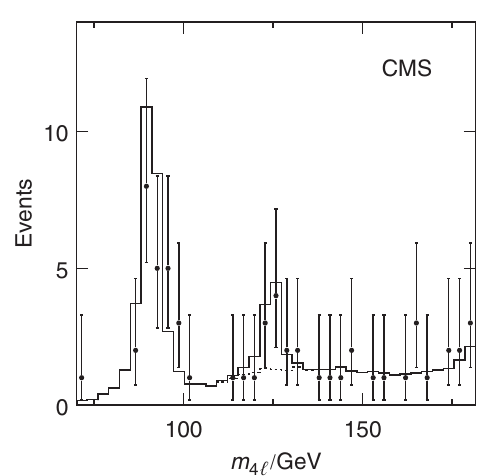
\includegraphics[scale=0.5]{Images/Z0peak.png}
\caption{The invariant 4-lepton-mass distribution. \textit{Thompson: Modern Particle Physics Fig. 17.19}}
\end{figure}
%See manual p. 41, also Thomson 17.19
\par There is a $Z^0$ peak (at $\approx 90$~GeV) and a Higgs-boson peak (at $\approx 125$~GeV). These come from the $Z^0 \, \rightarrow \, 4\ell$ and the $H^0 \, \rightarrow \, Z Z \, \rightarrow 4 \ell$ processes, respectively.  One example for the background at the Higgs-peak is the $t \rightarrow bW^+$ decay.\\[14pt]
\textit{Assume you have an ideal detector. What is the typical $\slashed{E}_T$ if a $Z^0$ pair has been produced and both $Z^0$ decay into electron or muon pairs? What $\slashed{E}_T$ will you expect when you have a real detector?}\\
\par In an ideal detector, there would be no missing energy in this process. In real detectors, there are energy losses not detected due to inactive detector elements, imperfect calibration.\\[14pt]
\textit{The Branching ratio of $t \, \rightarrow \, Wb$ is almost 100\%. If you have a top anti-top pair in an event, both particles decay instantly via $t \, \rightarrow \, bW$. If both W bosons each decay leptonically ($W \, \rightarrow \, \ell \nu$), one finds two leptons in the event. What could explain the occurence of four leptons in a $t \bar{t}$ event?}\\
\par The two top quarks can decay into b quarks and W bosons, both of which can further decay semi-leptonically. The process: 
\begin{equation}
t \bar{t} \, \rightarrow bW^+ \, \bar{b}W^- \, \rightarrow (l^- \ldots ) \, (\nu l^+) \, (l^+ \ldots) \, (l^- \bar{\nu})\nonumber
\end{equation}\\
\textit{Gedanken-experiment: given a histogram with 2000 bins of 20000 random integers between 1 and 2000, we expect an average of 100 entries per bin. What is the statistical error for the number of entries in one bin? What is the probability of finding a bin with 130 entries? How many of such 130 entries bins (in average) do you expect to appear in 200 bins? In other words, what is the probability to find a deviation of 3 standard deviations in one of the bins of the distribution?}\\
\par The error for bin entries is (counting statistics) $\sqrt{100} = 10$. Finding a bin with 130 entries (or more): $\sigma = 10 \Rightarrow 3\sigma$ is what we are looking for. The probability of higher than 130 or lower than 70 is $ 1- 3 \sigma = 1-0.9973$, so the requested probability for 1 bin is $(1-3\sigma)/2$. The probability that at least one of the bins has more than 130 counts:
\begin{equation}
P = 1 - \Big( 1 - \frac{1- 0.9973}{2} \Big)^{200} = 1-0.7532 = 0.2368.
\end{equation} 
\newpage
\end{document}